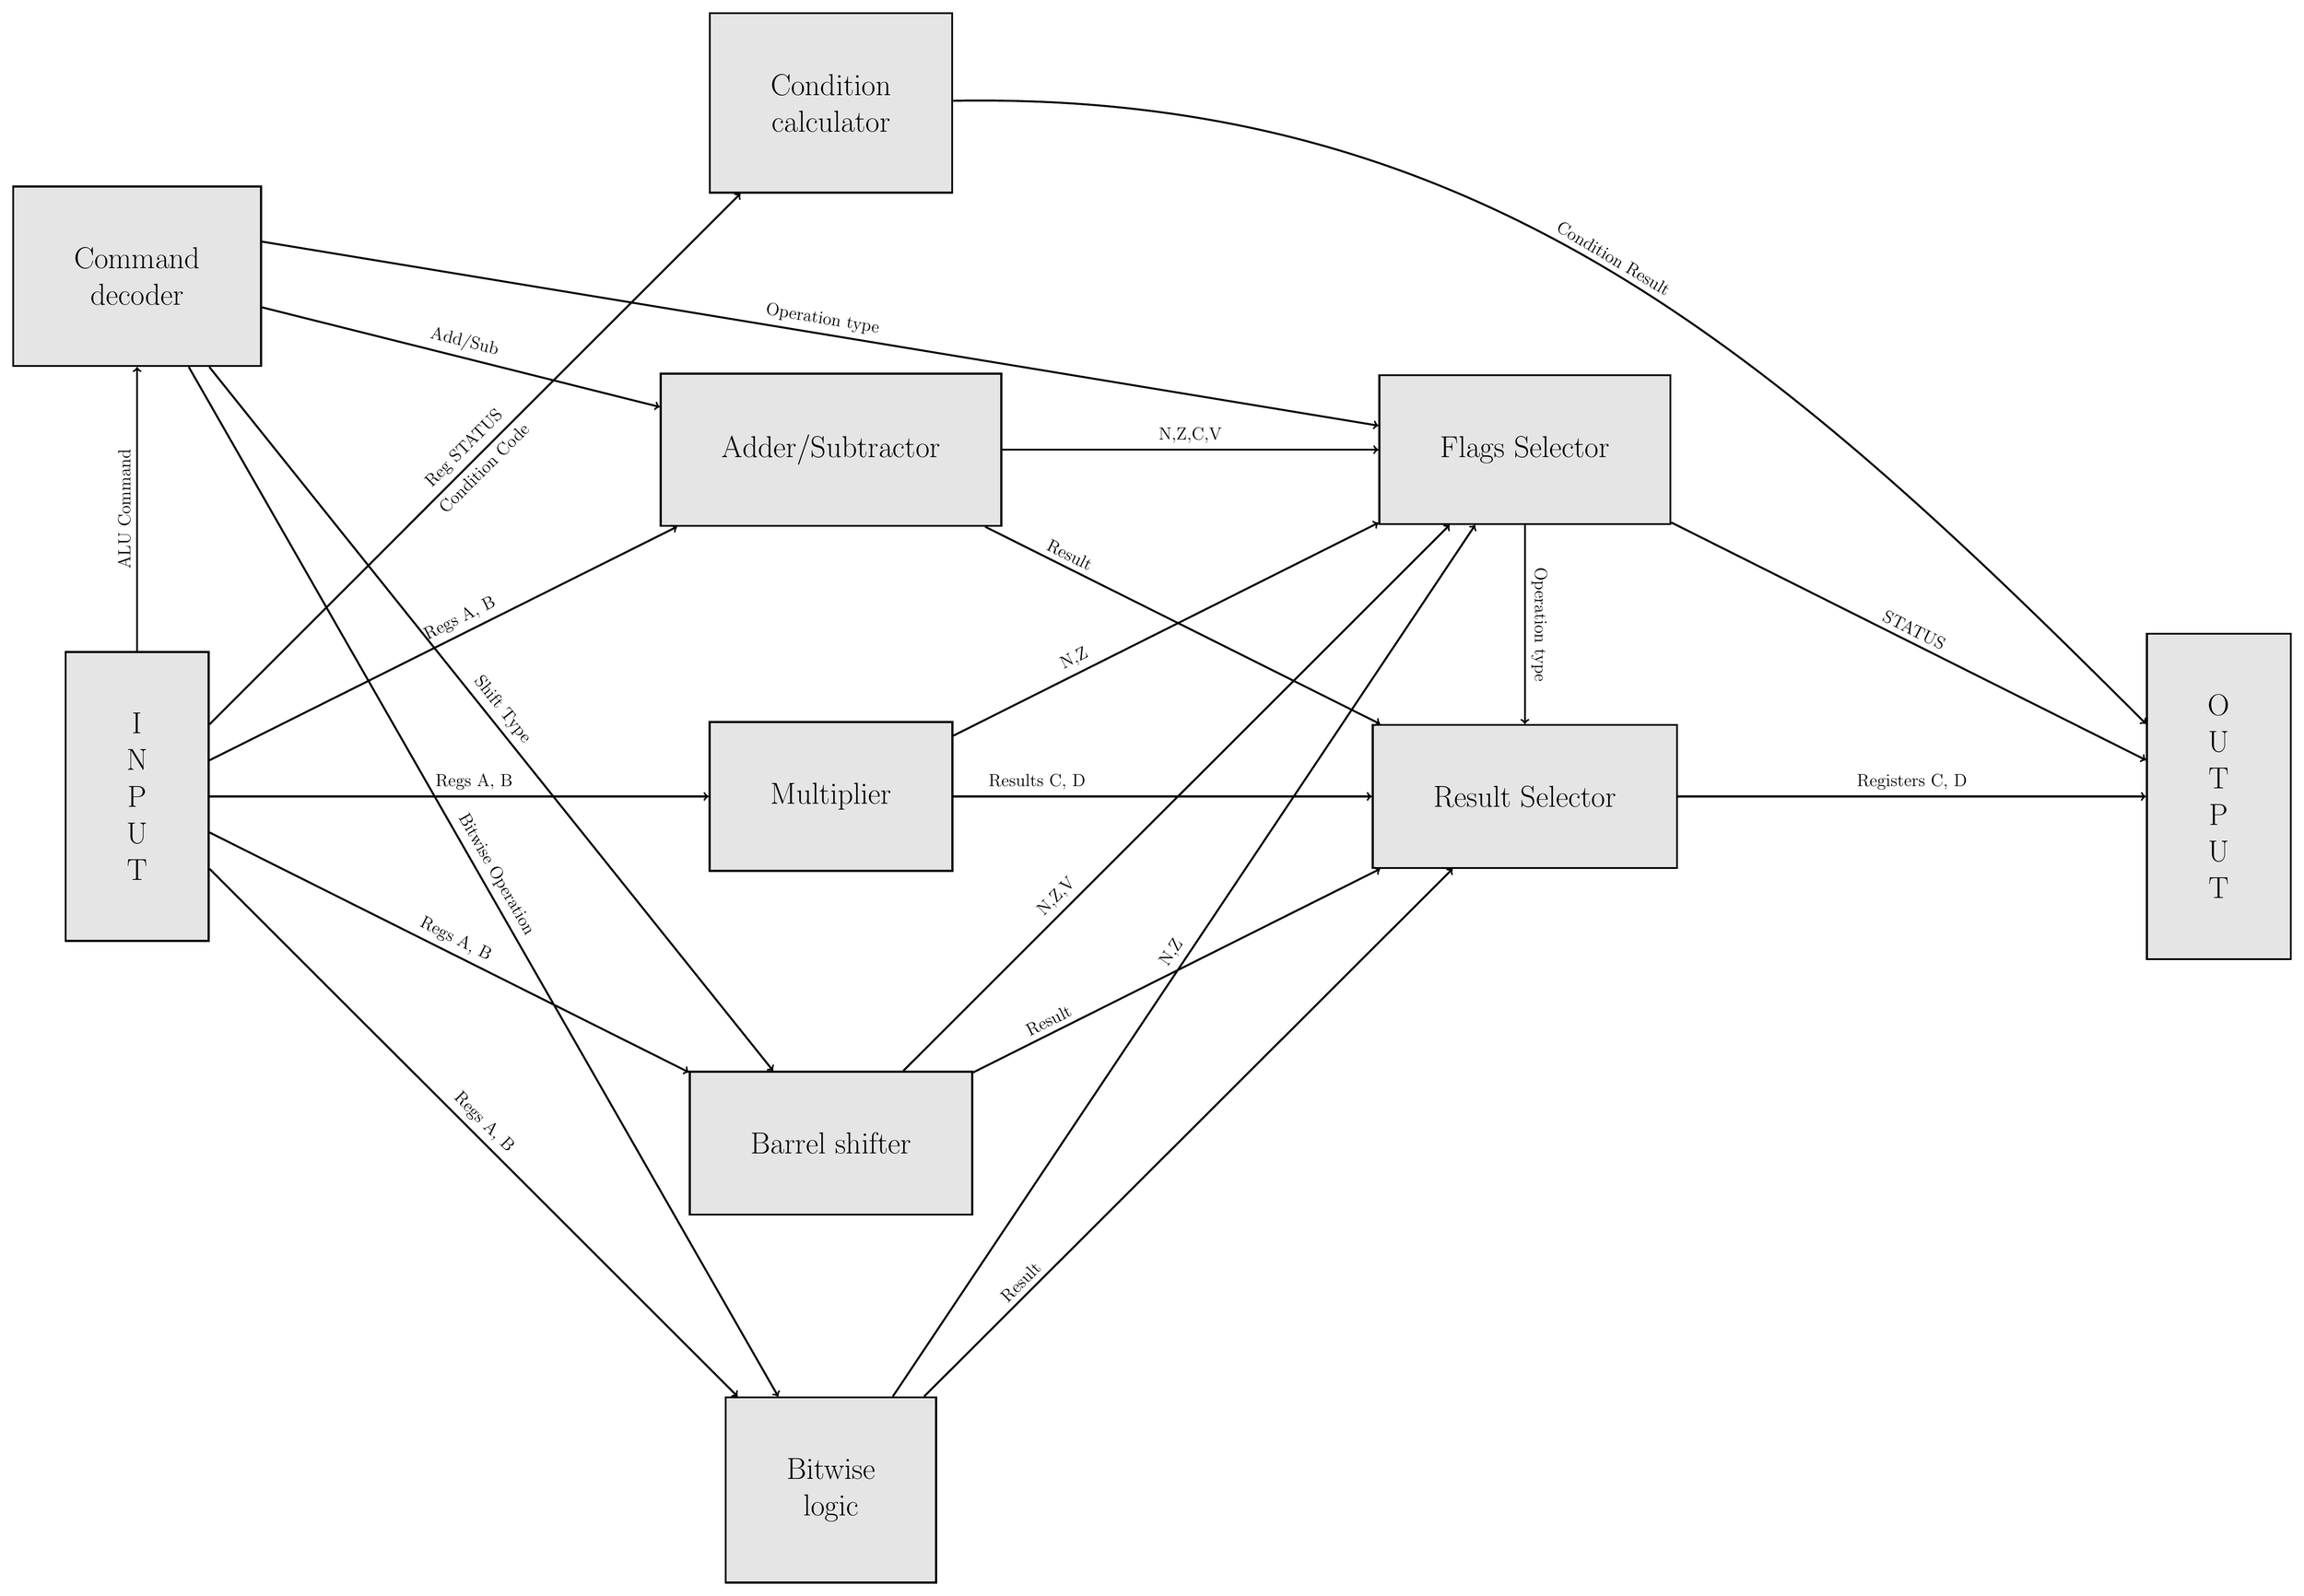
\begin{tikzpicture}[ultra thick, rect/.style={rectangle, draw=black,ultra thick, fill=gray!20, inner sep=#1, node font=\Huge, align=center}, rect/.default=50, arrownode/.style={pos=0.5, sloped, #1, node font=\Large}, arrownode/.default=above]

\node [rect] (IN) at (0, 0){I\\N\\P\\U\\T};
\node [rect] (CD) at (0, 15){Command \\decoder};
\node [rect] (ADD) at (20, 10){Adder/Subtractor};
\node [rect] (MUL) at (20, 0){Multiplier};
\node [rect] (BS) at (20, -10){Barrel shifter};
\node [rect] (BWS) at (20, -20){Bitwise\\logic};
\node [rect] (CC) at (20, 20){Condition\\calculator};
\node [rect] (FS) at (40, 10){Flags Selector};
\node [rect] (RS) at (40, 0){Result Selector};
\node [rect] (OUT) at (60,0){O\\U\\T\\P\\U\\T};

\draw[->,ultra thick] (IN) -- (CD) node [arrownode] {ALU Command};
\draw[->,ultra thick] (IN) -- (ADD) node [arrownode, pos=0.55] {Regs A, B}; 
\draw[->,ultra thick] (IN) -- (MUL) node [arrownode, pos=0.53] {Regs A, B};
\draw[->,ultra thick] (IN) -- (BS) node [arrownode] {Regs A, B};
\draw[->,ultra thick] (IN) -- (BWS) node [arrownode] {Regs A, B};
\draw[->,ultra thick] (IN) -- (CC) node [arrownode] {Reg STATUS} node [arrownode=below] {Condition Code};
\draw[->,ultra thick] (CD) -- (ADD) node [arrownode] {Add/Sub}; 
\draw[->,ultra thick] (CD) -- (BS) node [arrownode] {Shift Type};
\draw[->,ultra thick] (CD) -- (BWS) node [arrownode] {Bitwise Operation};  
\draw[->,ultra thick] (ADD) -- (FS) node [arrownode] {N,Z,C,V};
\draw[->,ultra thick] (MUL) -- (FS) node [arrownode,pos=0.3] {N,Z};
\draw[->,ultra thick] (BS) -- (FS) node [arrownode,pos=0.3] {N,Z,V};
\draw[->,ultra thick] (BWS) -- (FS) node [arrownode] {N,Z};
\draw[->,ultra thick] (ADD) -- (RS) node [arrownode,pos=0.2] {Result};
\draw[->,ultra thick] (MUL) -- (RS) node [arrownode,pos=0.2] {Results C, D};
\draw[->,ultra thick] (BS) -- (RS) node [arrownode,pos=0.2] {Result};
\draw[->,ultra thick] (BWS) -- (RS) node [arrownode,pos=0.2] {Result};
\draw[->,ultra thick] (CD.east)+(0,1) -- (FS) node [arrownode] {Operation type};
\draw[->,ultra thick] (FS) -- (RS) node [arrownode] {Operation type};
\draw[->,ultra thick] (FS) -- (OUT) node [arrownode] {STATUS};
\draw[->,ultra thick] (RS) -- (OUT) node [arrownode] {Registers C, D};
\draw[->,ultra thick] (CC) edge[out=1] node [arrownode] {Condition Result} (OUT) ;

\end{tikzpicture}